% Tento soubor nahraďte vlastním souborem s obsahem práce.
%=========================================================================
% Autoři: Michal Bidlo, Bohuslav Křena, Jaroslav Dytrych, Petr Veigend a Adam Herout 2019
\chapter{Úvod}
\label{chapter:uvod}

\chapter{Teorie}
Následující kapitola je věnována vysvětlení základní teorie skrývající se za simulacemi a animacemi tekutin a plynů. Nejprve je zde obecně vysvětlen pojem simulace a animace kapalin. Dále jsou zde vysvětleny různé přístupy k simulaci, je zde vysvětlena mřížková neboli Lagrangeova metoda a částicový přístup neboli Eulerova metoda. V každé sekci jsou následně popsány některé významné algoritmy spadající pod jednotlivé metody.

\label{chapter:teorie}
\section{Simulace kapalin}
Na začátek je nutné odlišit pojmy simulace kapalin a animace kapalin. V obou případech jde především o chování kapaliny v určité situaci, nicméně animace se oproti simulaci zaměřuje především na vizuální stránku a méně na fyzikální přesnost. Jedná se tedy pouze o aproximaci vzorců popisujících chování kapalin například zanedbáním velké části objemu kapaliny a popisem pouze chování hladiny kapaliny (viz níže). Jedním z možných využití takovýchto aproximací jsou případy, kde natolik nezáleží na přesnosti chování, jako spíše na vizuální stránce. Příkladem mohou být videohry, kde je nutné mít vizuálně přívětivou kapalinu, ale zároveň vypočitatelnou v reálném čase s přihlédnutím na výpočet mnoha dalších věcí v rámci herního enginu. Avšak například při tvorbě animací a vizuálních efektů pro filmy, kde nejsme omezeni časem, lze využívat mnohem výpočetně náročnějších animací. Tyto animace sice stále nemusí být fyzikálně dokonalé, avšak se jedná o mnohem propracovanější vyobrazení kapalin, než pouhé vlnění hladiny.

\begin{figure*}[h]\centering
  \centering
  \captionsetup{justification=centering}
  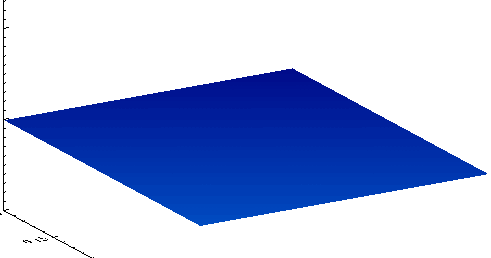
\includegraphics[width=0.3\linewidth]{obrazky-figures/SurfaceWaves/SurfWave_01.png}\hfill
  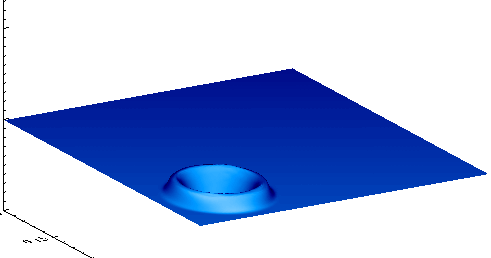
\includegraphics[width=0.3\linewidth]{obrazky-figures/SurfaceWaves/SurfWave_02.png}\hfill
  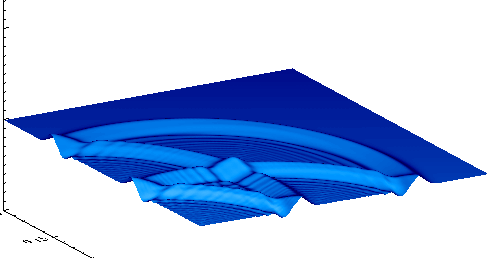
\includegraphics[width=0.3\linewidth]{obrazky-figures/SurfaceWaves/SurfWave_03.png}\hfill
  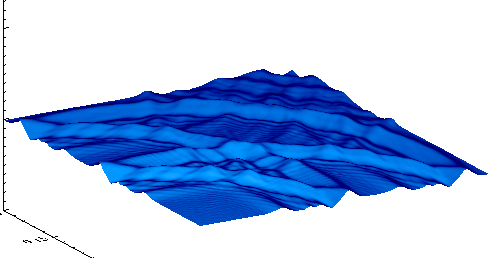
\includegraphics[width=0.3\linewidth]{obrazky-figures/SurfaceWaves/SurfWave_04.png}\hfill
  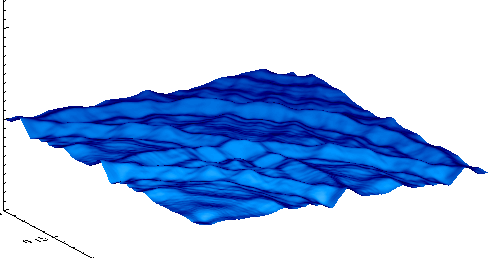
\includegraphics[width=0.3\linewidth]{obrazky-figures/SurfaceWaves/SurfWave_05.png}\hfill
  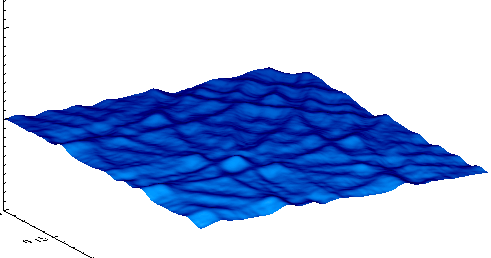
\includegraphics[width=0.3\linewidth]{obrazky-figures/SurfaceWaves/SurfWave_06.png}\hfill
  \caption{\textbf{Shallow Water Equation.} Postupné šíření vln při několika kapkách vody.}
  \textbf{Zdroj: } \url{https://en.wikipedia.org/wiki/Shallow_water_equations}
  \label{fig:SWE}
\end{figure*}

\subsubsection{Simulace hladiny}
Simulace vlnění hladiny je jedním z nejjednodušší vizualizace kapaliny. Existuje samozřejmě více přístupů jak takovou simulaci realizovat, mezi které patří například výškové mapy, vlnová funkce či rovnice mělké vody (Shallow Water Equation). Ačkoliv produkují v celku uspokojivé vlnění hladiny, existují v okolním světě běžné jevy, jako například lámající se vlny, které za pomocí jednoduchých vlnových funkcí a výškových map nelze simulovat.

\begin{figure}[hbt]
	\centering
	\captionsetup{justification=centering}
	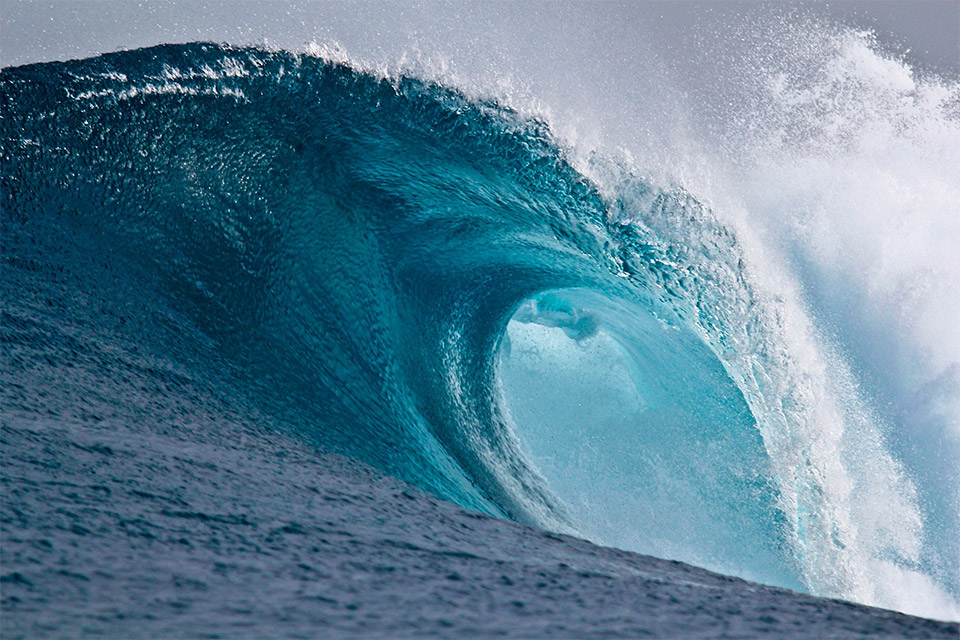
\includegraphics[width=0.4\textwidth]{obrazky-figures/Large_breaking_wave.jpg}
	\caption{\textbf{Lámající se vlna.} Jev v reálném světě, který není realizovatelný za pomocí výškových map a vlnových funkcí.}
	\textbf{Zdroj: } \url{https://en.wikipedia.org/wiki/Breaking_wave}
	\label{keepCalm}
\end{figure}

Simulace kapalin se naopak snaží být oproti animacím co nejvíce fyzikálně přesné, čímž ale rapidně vzrůstá náročnost výpočtů. Existuje nespočet metod jak dosáhnout výsledku, nicméně čím přesnější a složitější scéna tím delší výpočet daného scénáře. Doba výpočtu se tak může pohybovat v rámci minut, ale i hodin. Tyto metody jsou pak často založeny nad numerickými výpočty fyzikálních rovnic, kde nejpoužívanější rovnice jsou rovnice Navier-Stokes.

\subsection{Navier-Stokes rovnice}
Navier-Stokes rovnice jsou jedny z nejvyužívanějších rovnic pro výpočty chování kapalin. Základy pro popis dynamiky kapalin položil již v roce 1687 Sir Isaac Newton v článku "Principa", kde bylo poprvé správně popsáno chování viskózních kapalin. Později Daniel Bernoulli a Leonhard Euler popsali chování neviskózního toku pomocí rovnic dnes známých jako Eulerovy nevyskózní rovnice (Euler’s inviscid equations). Až Claude-Louis Navier a Sir George Stokes na sobě nezávisle odvodili finální podobu rovnic ze zmiňovaných Eulerových a Newtonových rovnic. Tyto Navier-Stokesovi rovnice jsou nyní nejpoužívanější formou popisu chování kapalin a bylo na nich postaveno nespočet různých algoritmů. \cite{simscale_2020}

\begin{equation}
	\rho(\frac{\partial}{\partial t} + \mathbf{u} \cdot \nabla)\mathbf{u} = -\nabla p + \mu\nabla\cdot(\nabla \mathbf{u}) + f 
	\label{eq:NavierStokes}
\end{equation}

\begin{equation}
	\nabla \cdot \mathbf{u} = 0
	\label{eq:NavierStokes2}
\end{equation}

Tři základní vlastnosti viskózní kapaliny, která má neměnné teplo, jsou rychlost ($\mathbf{u}$), tlak ($p$) a hustota ($\rho$). V rovnici \ref{eq:NavierStokes} pak $\mu$ označuje viskozitu kapaliny a $f$ ostatní síly působící na kapalinu, jako například gravitace. Tyto rovnice tak vyjadřují zákon o zachování hybnosti a zákon o zachování hmotnosti pro Newtonské kapaliny. Newtonosvksá kapalina je pak kapalina kterou lze popsat lineárním Newtonovým modelem. Její viskozita je pak závislá především na tlaku a teplotě a z tohoto hlediska se jedná o takzvanou Newtonovskou viskozitu. u Nenowtonské kapaliny pak popisujeme takzvanou zdánlivou viskozitu závislou na předchozí deformaci kapaliny a rychlosti vnitřního smyku kapaliny. Tyto kapaliny pak nelze popsat lineárním Newtonovým zákonem.\cite{StejskalJan2013Pmks}

Navier-Stokesovi rovnice jsou hojně využívány nejen pro simulaci a animaci kapalin, ale v celé řadě dalších vědních oborů. Využití můžeme nalézt při vytváření modelů pro předpověď počasí, při výrobě letadel pro studování toku vzduchu nebo například při analýze šíření znečištění.
\break

Existují dva úhly pohledu na organizaci a řešení nejen těchto rovnic, ale zároveň obecně dynamiky kapalin. Tyto metody se pak liší především v bodech pozorování. V Eulerově metodě dochází k výpočtu požadovaných hodnot v přesně daných bodech, tedy v nějaké diskrétní mřížce. U Lagrangeovy metody dochází k výpočtu v bodech sledované masy, tedy v částicích sledované kapaliny. Dále jsou obě metody detailněji popsány, včetně několika algoritmů, které pod dané metody spadají.

\begin{figure}[h]
\centering
\begin{subfigure}{.5\textwidth}
  	\centering
	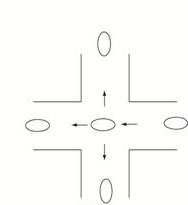
\includegraphics[width=0.7\linewidth]{obrazky-figures/EulerLagran_02.jpg}
	\caption{\textbf{Eulerův přístup}}
	\label{fig:Euler}
\end{subfigure}%
\begin{subfigure}{.5\textwidth}
  	\centering
	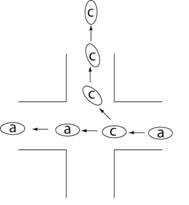
\includegraphics[width=0.7\linewidth]{obrazky-figures/EulerLagran_01.jpg}
	\caption{\textbf{Lagrangeův přístup}}
	\label{fig:Lagran}
\end{subfigure}
\caption{Příklad dvou přístupů nad křižovatkou s auty. Eulerův přístup (\ref{fig:Euler}) sleduje křižovatku v předem daných místech (ramena a střed křižovatky). Naopak Lagrangeův přístup(\ref{fig:Lagran}) sleduje konkrétní vozidla (a,c), jak projíždí křižovatkou.}
\textbf{Zdroj:} \url{http://abe-research.illinois.edu/faculty/dickc/Engineering/ELdescrip2a.htm}
\label{fig:ztencovani}
\end{figure}

\section{Eulerova metoda toku}
\subsection{Celulární automaty}
\subsection{Mřížková metoda}
\section{Lagrangeova metoda toku}
\subsection{Smoothed Particle Hydrodynamics}
\subsubsection{Weakly Compressible Smoothed Particle Hydrodynamics}
\subsubsection{Predictive-Corrective Incompressible Smoothed Particle Hydrodynamics}
\section{Hybridní přístup}




\chapter{Návrh řešení}
\label{chapter:navrh_resení}

\chapter{Implementace}
\label{chapter:implementace}

\chapter{Testování}
\label{chapter:testovani}

\chapter{Závěr}
\label{chapter:zaver}





%===============================================================================
